\documentclass[12pt, twoside]{article}
\usepackage[letterpaper, margin=1in, headsep=0.2in]{geometry}
\setlength{\headheight}{0.6in}
%\usepackage[english]{babel}
\usepackage[utf8]{inputenc}
\usepackage{microtype}
\usepackage{amsmath}
\usepackage{amssymb}
%\usepackage{amsfonts}
\usepackage{siunitx} %units in math. eg 20\milli\meter
\usepackage{yhmath} % for arcs, overparenth command
\usepackage{tikz} %graphics
\usetikzlibrary{quotes, angles}
\usepackage{graphicx} %consider setting \graphicspath{{images/}}
\usepackage{parskip} %no paragraph indent
\usepackage{enumitem}
\usepackage{multicol}
\usepackage{venndiagram}

\usepackage{fancyhdr}
\pagestyle{fancy}
\fancyhf{}
\renewcommand{\headrulewidth}{0pt} % disable the underline of the header
\raggedbottom
\hfuzz=2mm %suppresses overfull box warnings

\usepackage{hyperref}

\fancyhead[LE]{\thepage}
\fancyhead[RO]{\thepage \\ Name: \hspace{4cm} \,\\}
\fancyhead[LO]{BECA / Dr. Huson / Geometry\\*  Unit 6: Analytic geometry\\* 9 December 2022}

\begin{document}

\subsubsection*{6.2 Classwork: Linear equations \hfill 8.F.A.3}
The slope of a line: $\displaystyle m=\frac{y_2-y_1}{x_2-x_1}$
\begin{enumerate}
\item Find the slope of the line through the points $A(3,4)$, $B(9,8)$.
\begin{flushleft}
  \begin{tikzpicture}[scale=.65]
    \draw [help lines] (0,0) grid (10,9);
    \draw [thick, ->] (0,0) -- (10.4,0) node [below right] {$x$};
    \draw [thick, ->] (0,0)--(0,9.4) node [right] {$y$};
    \foreach \x in {1,...,10}
    \draw[shift={(\x,0)}] (0pt,-3pt)--(0pt,3pt) node[below=5pt] {$\x$};
    \foreach \y in {1,...,9}
    \draw[shift={(0,\y)}] (-3pt,0pt)--(3pt,0pt) node[left=5pt] {$\y$};
    \draw [thick, <->] (-1,1.33)--(9.5,8.33);
    \draw [fill] (3,4) circle [radius=0.08] node[above left] {$A$};
    \draw [fill] (9,8) circle [radius=0.08] node[above left] {$B$};
  \end{tikzpicture}
  \end{flushleft}

\subsubsection*{The slope-intercept equation of a line}
$y=mx+b$, where $m$ is the slope and $b$ is the $y$-intercept
\item The line $l$ has the equation $y=\frac{3}{2}x-1$. 
\begin{enumerate}
  \item Write down it's slope and $y$-intercept. \hspace{2cm} $m=$
  \hspace{2cm} $b=$
  \item Is the point $(4, 4)$ on the line $l$? Justify your answer.
\end{enumerate}
\vspace{2cm}

\item A line is shown on the grid below.
\begin{multicols}{2}
\begin{enumerate}
  \item Write down it's slope, $y$-intercept.\\ $m=$
  \hspace{2cm} $b=$
  \vspace{0.25cm}
  \item Write down the equation of the line.
  \vspace{1cm}
  \item State the coordinates of the point $P$.
\end{enumerate}
  \begin{center}
  \begin{tikzpicture}[scale=0.7]
    \draw [help lines] (-3,-1) grid (4,6);
    \draw [thick, ->] (-3.2,0) -- (4.4,0) node [below right] {$x$};
    \draw [thick, ->] (0,-1.2)--(0,6.4) node [left] {$y$};
    \foreach \x in {-3, -2, ..., 4} \draw (\x cm,1pt) -- (\x cm,-1pt) node[anchor=north] {$\x$};
    \foreach \y in {1, 2, 3, 4, 5} \draw (1pt,\y cm) -- (-1pt,\y cm) node[anchor=east] {$\y$};
    \draw [thick, <->] (-3.5,-1.5) -- (4.2,6.2);
    \fill (3,5) circle[radius=0.1] node[below right]{$P$};
  \end{tikzpicture}
  \end{center}
\end{multicols}

\newpage
\item Draw a straight line through the points $A$ and $B$ shown on the grid below.
\begin{multicols}{2}
\begin{enumerate}
  \item Write down the line's $y$-intercept.\\ $b=$
  \vspace{0.25cm}
  \item Write down the slope of the line.\\ $m=$
  \vspace{0.25cm}
  \item Write down the equation of the line.
\end{enumerate}
  \begin{center} %4 quadrant regents grid w T-Chart
  \begin{tikzpicture}[scale=0.8]
    %\draw [help lines] (-3,-2) grid (4,6);
    \draw [thick, ->] (-3.2,0) -- (5.4,0) node [below right] {$x$};
    \draw [thick, ->] (0,-1.2)--(0,6.4) node [left] {$y$};
    \foreach \x in {-2, -1, ..., 5} \draw (\x cm,3pt) -- (\x cm,-3pt) node[anchor=north] {$\x$};
    \foreach \y in {1, 2, 3, 4, 5} \draw (3pt,\y cm) -- (-3pt,\y cm) node[anchor=east] {$\y$};
    %\draw [thick, <->] (-3.5,-1.5) -- (4.2,6.2);
    \fill (0,4) circle[radius=0.1] node[above right]{$A (0,4)$};
    \fill (4,2) circle[radius=0.1] node[above right]{$B (4,2)$};
  \end{tikzpicture}
  \end{center}
\end{multicols}
\vspace{1cm}

\item Find the slope of the line through the points $(-1, 3)$ and $(5, 0)$. \vspace{3cm}

\item A linear equation is graphed below.
\begin{multicols}{2}
\begin{enumerate}
  \item State the coordinates of the point $A$. \vspace{0.25cm}
  \item Write down the line's slope.\\ $m=$
  \vspace{0.25cm}
  \item Write down it's $y$-intercept.\\ $b=$
  \vspace{0.25cm}
  \item Write down the equation of the line.
  \vspace{1cm}
  \item Find the $x$-intercept.
\end{enumerate} \vspace{.5cm}
  \begin{center} 
  \begin{tikzpicture}[scale=0.8]
    \draw [help lines] (-2,-2) grid (5,6);
    \draw [thick, ->] (-2.2,0) -- (5.4,0) node [below right] {$x$};
    \draw [thick, ->] (0,-2.2)--(0,6.4) node [left] {$y$};
    \foreach \x in {-2,-1,1,2,...,5} \draw (\x cm,1pt) -- (\x cm,-1pt) node[anchor=north] {$\x$};
    \foreach \y in {1, 2, 3, 4, 5} \draw (1pt,\y cm) -- (-1pt,\y cm) node[anchor=east] {$\y$};
    \draw [thick, <->,domain=-1:4.5] plot(\x,3/2*\x-1);
    \fill (4,5) circle[radius=0.1] node[above left]{$A$};
  \end{tikzpicture}
  \end{center}
\end{multicols} \vspace{1cm}

\newpage
\subsubsection*{The slope of a line}
``rise over run'': $\displaystyle m=\frac{y_2-y_1}{x_2-x_1}$

\item Find the slope of the line through the points $A(2,3)$, $B(8,5)$.
\begin{flushleft}
  \begin{tikzpicture}[scale=.65]
    \draw [help lines] (0,0) grid (10,10);
    \draw [thick, ->] (0,0) -- (10.4,0) node [below right] {$x$};
    \draw [thick, ->] (0,0)--(0,10.4) node [right] {$y$};
    \foreach \x in {1,...,10}
    \draw[shift={(\x,0)}] (0pt,-3pt)--(0pt,3pt) node[below=5pt] {$\x$};
    \foreach \y in {1,...,10}
    \draw[shift={(0,\y)}] (-3pt,0pt)--(3pt,0pt) node[left=5pt] {$\y$};
    \draw [thick, <->] (0.5,2.5)--(9.5,5.5);
    \draw [fill] (2,3) circle [radius=0.08] node[above left] {$A$};
    \draw [fill] (8,5) circle [radius=0.08] node[above left] {$B$};
  \end{tikzpicture}
  \end{flushleft}

\item Two lines are graphed below. 
\begin{enumerate}
  \item Complete the T-tables for each.
  \item Write down the equations for each.
\end{enumerate}
  \begin{center} 
  \begin{tikzpicture}[scale=0.8]
    \draw [help lines] (-3,-2) grid (6,6);
    \draw [thick, ->] (-3.2,0) -- (6.4,0) node [below right] {$x$};
    \draw [thick, ->] (0,-2.2)--(0,6.4) node [left] {$y$};
    \foreach \x in {-3,-2,-1,1,2,...,6} \draw (\x cm,1pt) -- (\x cm,-1pt) node[anchor=north] {$\x$};
    \foreach \y in {-1,1, 2, 3, 4, 5} \draw (1pt,\y cm) -- (-1pt,\y cm) node[anchor=east] {$\y$};

    \draw [thick, <->,samples=20,domain=-2.5:5.5] plot(\x,0.5*\x+1);
    \node at (5.7,3.3){$f$};
    \draw [thick, <->,samples=20,domain=-1.5:5.5] plot(\x,-1*\x+4);
    \node at (-1.5,4.5){$g$};

    \draw [thick] (-7,-1) -- (-7,6);
    \draw [thick] (-8.5,5) -- (-5.5,5);
    \node at (-7,7){$f(x)$};
    \node at (-8,5.5){$x$};
    \node at (-6,5.5){$y$};
    \draw [thick] (9,-1) -- (9,6);
    \draw [thick] (7.5,5) -- (10.5,5);
    \node at (9,7){$g(x)$};
    \node at (-8,4){$-2$}; 
    \node at (-8,2.5){$0$}; 
    \node at (-8,1){$2$}; 
    \node at (-6,-0.5){$3$};
    \fill (-2,0) circle[radius=0.1];
    \fill (0,1) circle[radius=0.1];
    \fill (2,2) circle[radius=0.1];
    \fill (4,3) circle[radius=0.1];
  \end{tikzpicture}
  \end{center}

\item The line $l$ is graphed at right.
  \begin{multicols}{2}
  \begin{enumerate}
    \item Write down the line's slope.\\ $m=$
    \vspace{0.5cm}
    \item Write down it's $y$-intercept.\\ $b=$
    \vspace{0.5cm}
    \item Write down the equation of the line.
    \vspace{1.5cm}
    \item Draw a line parallel to $l$ through point $P$. (use a straight edge for full credit)
  \end{enumerate} \vspace{.5cm}
    \begin{center} 
    \begin{tikzpicture}[scale=0.8]
      \draw [help lines] (-2,-1) grid (5,6);
      \draw [thick, ->] (-2.2,0) -- (5.4,0) node [below right] {$x$};
      \draw [thick, ->] (0,-1.2)--(0,6.4) node [left] {$y$};
      \foreach \x in {-2,-1,1,2,...,5} \draw (\x cm,1pt) -- (\x cm,-1pt) node[anchor=north] {$\x$};
      \foreach \y in {1, 2, 3, 4, 5} \draw (1pt,\y cm) -- (-1pt,\y cm) node[anchor=east] {$\y$};
      \draw [thick, <->] (-1.5,2.5) -- (4.5,4.5)node[right]{$l$};
      \fill (3,2) circle[radius=0.1] node[below right]{$P$};
    \end{tikzpicture}
    \end{center}
  \end{multicols}
  
\item Write the linear equation $\displaystyle y-5=\frac{2}{3}(x-3)$ in the form $y=mx+c$. \vspace{4cm}
  
\newpage
\item Two lines are graphed below. 
  \begin{enumerate}
    \item Complete the T-tables for each.
    \item Write down the equations for each.
  \end{enumerate}
    \begin{center} 
    \begin{tikzpicture}[scale=0.8]
      \draw [help lines] (-3,-2) grid (6,6);
      \draw [thick, ->] (-3.2,0) -- (6.4,0) node [below right] {$x$};
      \draw [thick, ->] (0,-2.2)--(0,6.4) node [left] {$y$};
      \foreach \x in {-3,-2,-1,1,2,...,6} \draw (\x cm,1pt) -- (\x cm,-1pt) node[anchor=north] {$\x$};
      \foreach \y in {-1,1, 2, 3, 4, 5} \draw (1pt,\y cm) -- (-1pt,\y cm) node[anchor=east] {$\y$};
  
      \draw [thick, <->,samples=20,domain=-2.5:5.5] plot(\x,0.5*\x+1);
      \node at (5.7,3.3){$f$};
      \draw [thick, <->,samples=20,domain=-1.5:5.5] plot(\x,-1*\x+4);
      \node at (-1.5,4.5){$g$};
  
      \draw [thick] (-7,-1) -- (-7,6);
      \draw [thick] (-8.5,5) -- (-5.5,5);
      \node at (-7,7){$f(x)$};
      \node at (-8,5.5){$x$};
      \node at (-6,5.5){$y$};
      \draw [thick] (9,-1) -- (9,6);
      \draw [thick] (7.5,5) -- (10.5,5);
      \node at (9,7){$g(x)$};
      \node at (-8,4){$-2$}; 
      \node at (-8,2.5){$0$}; 
      \node at (-8,1){$2$}; 
      \node at (-6,-0.5){$3$};
      \fill (-2,0) circle[radius=0.1];
      \fill (0,1) circle[radius=0.1];
      \fill (2,2) circle[radius=0.1];
      \fill (4,3) circle[radius=0.1];
    \end{tikzpicture}
    \end{center}

\item The line $l$ is graphed at right.
  \begin{multicols}{2}
  \begin{enumerate}
    \item Write down the line's slope.\\ $m=$
    \vspace{0.5cm}
    \item Write down it's $y$-intercept.\\ $b=$
    \vspace{0.5cm}
    \item Write down the equation of the line.
    \vspace{1.5cm}
    \item Draw a line parallel to $l$ through point $P$. (use a straight edge for full credit)
  \end{enumerate} \vspace{.5cm}
    \begin{center} 
    \begin{tikzpicture}[scale=0.8]
      \draw [help lines] (-2,-1) grid (5,6);
      \draw [thick, ->] (-2.2,0) -- (5.4,0) node [below right] {$x$};
      \draw [thick, ->] (0,-1.2)--(0,6.4) node [left] {$y$};
      \foreach \x in {-2,-1,1,2,...,5} \draw (\x cm,1pt) -- (\x cm,-1pt) node[anchor=north] {$\x$};
      \foreach \y in {1, 2, 3, 4, 5} \draw (1pt,\y cm) -- (-1pt,\y cm) node[anchor=east] {$\y$};
      \draw [thick, <->] (-1.5,0.5) -- (3.5,5.5)node[right]{$l$};
      \fill (3,3) circle[radius=0.1] node[below right]{$P$};
    \end{tikzpicture}
    \end{center}
  \end{multicols}

\item Find the slope of the line through the points $(3, -2)$ and $(-3, 2)$. \vspace{4cm}

\item Write the linear equation $\displaystyle y-5=\frac{2}{5}(x-10)$ in the form $y=mx+c$. \vspace{4cm}

\item Is the point $(-4,1)$ on the line $\displaystyle y=\frac{1}{2}x+3$? Support your answer algebraically.

\newpage
\item Two lines are graphed below. 
\begin{enumerate}
  \item Complete the T-tables for each.
  \item Write down the equations for each.
\end{enumerate}
  \begin{center} 
  \begin{tikzpicture}[scale=0.8]
    \draw [help lines] (-3,-2) grid (6,6);
    \draw [thick, ->] (-3.2,0) -- (6.4,0) node [below right] {$x$};
    \draw [thick, ->] (0,-2.2)--(0,6.4) node [left] {$y$};
    \foreach \x in {-3,-2,-1,1,2,...,6} \draw (\x cm,1pt) -- (\x cm,-1pt) node[anchor=north] {$\x$};
    \foreach \y in {-1,1, 2, 3, 4, 5} \draw (1pt,\y cm) -- (-1pt,\y cm) node[anchor=east] {$\y$};

    \draw [thick, <->,samples=20,domain=-2.5:5.5] plot(\x,0.5*\x+2);
    \node at (5.7,4.3){$f$};
    \draw [thick, <->,samples=20,domain=-1.5:5.5] plot(\x,-0.5*\x+4);
    \node at (-1.75,4.25){$g$};

    \draw [thick] (-7,-1) -- (-7,6);
    \draw [thick] (-8.5,5) -- (-5.5,5);
    \node at (-7,7){$f(x)$};
    \node at (-8,5.5){$x$};
    \node at (-6,5.5){$y$};
    \draw [thick] (9,-1) -- (9,6);
    \draw [thick] (7.5,5) -- (10.5,5);
    \node at (9,7){$g(x)$};
    \node at (-8,4){$-2$}; 
    \node at (-8,2.5){$0$}; 
    \node at (-8,1){$2$}; 
    \node at (-6,-0.5){$4$};
    \fill (-2,1) circle[radius=0.1];
    \fill (0,2) circle[radius=0.1];
    \fill (2,3) circle[radius=0.1];
    \fill (4,4) circle[radius=0.1];
  \end{tikzpicture}
  \end{center}


    
\end{enumerate}
\end{document}